
\chapter[Nguyên tắc thông tin liên lạc\\ bằng sóng vô tuyến]{Nguyên tắc thông tin liên lạc bằng sóng vô tuyến}
\section{Lý thuyết}
\subsection {Nguyên tắc chung của việc thông tin liên lạc bằng sóng vô tuyến}
\begin{itemize}
	\item Dùng sóng điện từ cao tần.
	\item Biến điệu sóng mang.
	\item Tách sóng.
	\item Khuếch đại.
\end{itemize}
\subsection {Sơ đồ khối của máy phát thanh vô tuyến đơn giản}
\begin{center}
	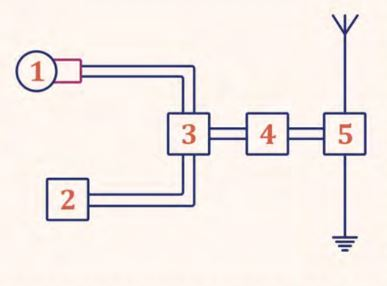
\includegraphics[scale=0.5]{../figs/4-4-1.JPG}
\end{center}
\begin{enumerate}
	\item \bltext{Micrô.}
	\item \bltext{Mạch tách sóng điện từ cao tần.}
	\item \bltext{ Mạch biến điệu (trộn sóng điện từ).}
	\item \bltext{ Mạch khuếch đại.}
	\item  \bltext{Anten phát.}
\end{enumerate}
\subsection {Sơ đồ khối của một máy thu thanh vô tuyến đơn giản}
\begin{center}
	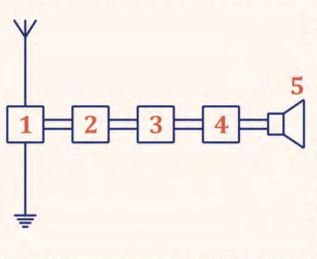
\includegraphics[scale=0.7]{../figs/4-4-2.JPG}
\end{center}
\begin{enumerate}
	\item \bltext{Anten thu.}
	\item \bltext{Mạch khuếch đại điện từ cao tần.}
	\item \bltext{Mạch tách sóng.}
	\item \bltext{Mạch khuếch đại dao động điện từ âm tần.}
	\item \bltext{Loa.}
\end{enumerate}
\subsection {Ứng dụng của sóng điện từ}
Sóng vô tuyến điện dùng để tải các thông tin, âm thanh và hình ảnh. Nhờ đó con người có thể thông tin liên lạc từ vị trí này đến vị trí khác trên mặt đất và trong không gian mà không cần dây dẫn.
\section{Bài tập tự luyện}
\begin{enumerate}[label=\bfseries Câu \arabic*:]
	
	%=======================	
	\item \mkstar{1} [1]
	\cauhoi
	{Máy phát thanh vô tuyến đơn giản không có bộ phận nào sau đây?
		\begin{mcq}(4)
			\item Mạch biến điệu.
			\item Micro.
			\item Mạch tách sóng.
			\item Mạch khuếch đại.
		\end{mcq}
	}
	
	\loigiai
	{		\textbf{Đáp án: C.}
		
		Máy phát thanh vô tuyến đơn giản không có bộ phận mạch tách sóng.
	} 
	
	%=======================    	
	\item \mkstar{1} [1]
	\cauhoi
	{Sóng vô tuyến điện không bị tần điện li hấp thụ, phản xạ và truyền thẳng qua được tầng điện li có bước sóng là
		\begin{mcq}(4)
			\item $\SI{20}{m}$.
			\item $\SI{2}{m}$. 
			\item $\SI{2000}{m}$. 
			\item $\SI{200}{m}$. 
		\end{mcq}
	}
	
	\loigiai
	{		\textbf{Đáp án: B.}
		
		Sóng vô tuyến không bị tần điện li hấp thụ, phản xạ và truyền thẳng qua được tầng điện li là sóng cực ngắn có bước sóng vào cỡ vài mét.
		
	}
	
	%=======================	
	\item \mkstar{1} [3]
	\cauhoi
	{Ở đảo Song Tử Tây (là đảo lớn thứ hai của quần đảo Trường Sa do Việt Nam quản lí), để có thể xem được các chương trình truyền hình phát sóng qua vệ tinh, người ta dùng anten thu sóng trực tiếp từ vệ tinh, qua bộ xử lí tín hiệu rồi đưa ra màn hình. Sóng điện từ mà anten trực tiếp thu từ vệ tinh là loại 
		\begin{mcq}(4)
			\item sóng ngắn. 
			\item sóng cực ngắn. 
			\item sóng trung. 
			\item sóng dài. 
		\end{mcq}
	}
	
	\loigiai
	{		\textbf{Đáp án: B.}
		
		Sóng vô tuyến dùng để truyền phát tín hiệu qua vệ tinh là sóng cực ngắn.
		
	}
	
	%=======================	
	\item \mkstar{1} [7]
	\cauhoi
	{Trong “máy bắn tốc độ” của cảnh sát giao thông sử dụng để đo tốc độ của phương tiện giao thông
		\begin{mcq}(1)
			\item chỉ có máy thu sóng vô tuyến.	
			\item có cả máy phát và thu sóng vô tuyến.
			\item chỉ có máy phát sóng vô tuyến.	
			\item không có máy phát và thu sóng vô tuyến.
		\end{mcq}
	}
	
	\loigiai
	{		\textbf{Đáp án: B.}
		
		Trong “máy bắn tốc độ” của cảnh sát giao thông sử dụng để đo tốc độ của phương tiện giao thông có cả máy phát và thu sóng vô tuyến.
		
	}
	
	%=======================	
	\item \mkstar{1} [9]
	\cauhoi
	{Khi sử dụng máy thu thanh vô tuyến điện, người ta vặn nút dò đài là để
		\begin{mcq}(1)
			\item thay đổi tần số của sóng tới. 
			\item tách tín hiệu cần thu ra khỏi sóng mang cao tần.
			\item thay đổi tần số riêng của mạch chọn sóng.
			\item khuếch đại tín hiệu thu được.
		\end{mcq}
	}
	
	\loigiai
	{		\textbf{Đáp án: C.}
		
		Khi sử dụng máy thu thanh vô tuyến điện, người ta vặn nút dò đài là để thay đổi tần số riêng của mạch chọn sóng.
		
	}
	
	%=======================	
	\item \mkstar{1} [9]
	\cauhoi
	{Trong sơ đồ của một máy phát sóng vô tuyến điện không có mạch
		\begin{mcq}(2)
			\item biến điệu. 
			\item khuếch đại. 
			\item tách sóng. 
			\item phát động cao tần. 
		\end{mcq}
	}
	
	\loigiai
	{		\textbf{Đáp án: C.}
		
		Trong sơ đồ của một máy phát sóng vô tuyến điện không có mạch tách sóng. 
		
	}
	
	%=======================
	\item \mkstar{3} [10]
	\cauhoi
	{Một mạch dao động ở máy vào của một máy thu thanh gồm cuộn thuần cảm có độ tự cảm $\SI{3}{\mu H}$ và tụ điện có điện dung biến thiên trong khoảng từ $\SI{10}{pF}$ đến $ \SI{500}{pF} $ . Biết rằng, muốn thu được sóng điện từ thì tần số riêng của mạch dao động phải bằng tần số của sóng điện từ cần thu (để có cộng hưởng). Trong không khí, tốc độ truyền sóng điện từ là $ \xsi{3.10^{8}}{m/s} $, máy thu này có thể thu được sóng điện từ có bước sóng trong khoảng
		
		\begin{mcq}(2)
			\item từ $ \SI{100}{m} $ đến $ \SI{730}{m} $.
			\item từ $ \SI{10,32}{m} $ đến $ \SI{73}{m} $.
			\item từ $ \SI{1,24}{m} $ đến $ \SI{73}{m} $.
			\item từ $ \SI{10}{m} $ đến $ \SI{730}{m} $. 
		\end{mcq}
	}
	
	\loigiai
	{		\textbf{Đáp án: B.}
		
		Bước sóng của mạch dao động cho bời:
		$$
		\lambda=2 \pi c \sqrt{L C}.
		$$
		Với $C_{1}=10 p F$, ta thu được bước sóng
		$$
		\lambda_{1}=2 \pi c \sqrt{L C_{1}}=2 \pi \cdot 3.10^{8} \sqrt{3.10^{-6} \cdot 10.10^{-12}}= \SI{10,32}{m}.
		$$
		Với $C_{2}=500 p F$, ta thu được bước sóng
		$$
		\lambda_{1}=2 \pi c \sqrt{L C_{2}}=2 \pi \cdot 3.10^{8} \sqrt{3.10^{-6} \cdot 500.10^{-12}}= \SI{73}{m}.
		$$
		Vậy máy này có thể thu được bước sóng trong khoảng từ $\SI{10,32}{m}$ đến \SI{73}{m}.
		
	}
	
\end{enumerate}
